\documentclass[12pt]{exam}

\usepackage{graphicx} % allows for graphics
\usepackage{ifthen}  % for if statements 

\newcommand{\sol}{1} %solution =1 or 0

% LOAD PACKAGES
\usepackage{amsmath} % allows for align env and other things
\usepackage{amssymb} % 
\usepackage{mathtools} % allows for single apostrophe
\usepackage{enumitem} % allows for alpha lettering in enumerated lists
\usepackage{lastpage}
\usepackage{array} % for table alignments
\usepackage{graphicx} % if images are needed

\addpoints

\usepackage{pgfplots} % for surfaces (chapter 7)
\usepackage{tikz-3dplot} 
\pgfplotsset{compat=1.9}
\usetikzlibrary{decorations.pathmorphing,patterns} % for some tikz diagrams
% ~~~~~~~~~~~~~~~~~~~~~~~~~~~~~~~~~~~~
% INITIALS
\newcommand{\Initials}{\textit{\Course, \TestName. Your initials: \underline{\hspace{3cm}}} \vspace{1pt}}

\newcommand{\InitialsLeft}{\noindent \hspace{-18pt}\textit{\Course, \TestName. Your initials: \underline{\hspace{3cm}}} \vspace{1pt}}

\newcommand{\InitialsRight}{\begin{flushright}\textit{\Course, \TestName. Your initials: \underline{\hspace{3cm}}} \vspace{1pt}\end{flushright}}

% ~~~~~~~~~~~~~~~~~~~~~~~~~~~~~~~~~~~~
% INSTRUCTIONS FOR DISTANCE LEARNING WITH NO PROCTOR
\newcommand{\InstructionsFormatAndTiming}{

    \begin{itemize} \setlength\itemsep{.1em}
    
        % \item You should only need 75 min to take the exam, but students will have \Duration to submit the exam, from the time that it is released.
        
        \item {\bf Show your work} and justify your answers for all questions unless stated otherwise.
        
        \item Please write neatly, and use dark and clear writing so that the scan is easy to read. 
        
        \item Please solve the questions in the exam in the order they are given. 
        
        \item You do not need to print the exam. As long as you solve problems in the order they are given you can write your answers on your own paper or by using a tablet. But students can print the exam and write their answers on the printed copy if they prefer. 

        \item Do not type your answers to any part of the exam. 
        
    \end{itemize}

}

\newcommand{\InstructionsSubmission}{

    \begin{itemize} \setlength\itemsep{.1em}
        \item Students should scan their work and submit it through Gradescope. There should be an \textbf{assignment} in Gradescope for this exam. 
        
        \item Work must be submitted by \DueDate. 
        
        \item Please upload your work as a single file. 
        
        \item During the upload process in Gradescope, please indicate which page of your work corresponds to each question. A small number of points will be allocated for this.
    \end{itemize}
}

\newcommand{\InstructionsQuestions}{

    \begin{itemize} \setlength\itemsep{.1em}
        
        \item If there are questions during the exam, students can email their instructor or message them through Canvas. 
        
        \item Our course Piazza forum will be temporarily inactive during the exam. 
        
        \item If you run into any technical issues or any unanticipated emergencies, please email your instructor as soon as you can. 
    
        
    \end{itemize}

}


\newcommand{\InstructionsHonor}{

    \begin{itemize} \setlength\itemsep{.1em}    
        \item Students can use any resources while taking these tests including online calculators and Mathematica
        \item Students cannot communicate with anyone during these tests.
        \item Students cannot use solutions provided from another student or third party. 
        \item In other words: do your own work but you can use technology to solve problems. 
 
    \end{itemize}

}






\newcommand{\GTHonorCode}{Having read the Georgia Institute of Technology Academic Honor Code, I understand and accept my responsibility as a member of the Georgia Tech community to uphold the Honor Code at all times. }



% FANCY HEADERS - MAKE EMPTY
\pagestyle{headandfoot}
\runningfooter{}{}{}


% ADJUST MARGINS FOR DISTANCE LEARNING REQUIREMENTS
\usepackage[tmargin=1.0in,bmargin=1.0in,left=1in,right=1in]{geometry}


% TIKZ DIAGRAMS
\usepackage{color}
\usepackage{tikz}  \usetikzlibrary{arrows} 
\usetikzlibrary{calc} 


% ADJUST FIRST LINE IN PARAGRAPH INDENTATION 
\setlength\parindent{0pt}


% COURSE SPECIFIC INFORMATION
\newcommand{\Course}{Math 2552}
\newcommand{\Instructors}{}

% WHO TO CONTACT DURING EXAM IF QUESTIONS
\newcommand{\InstructorContact}{}

\usepackage{spalign} % Joe Rabinoff's matrix package

\newcommand{\LastPage}{\begin{center}\textit{This page may be used for scratch work. Please indicate clearly if you would like your work on this page to be graded. }\end{center}   }


% DERIVATIVES
\newcommand{\dydt}{{\frac{dy}{dt}}} % 
\newcommand{\dydx}{{\frac{dy}{dx}}} % 
\newcommand{\dydtt}{{\frac{d ^2y}{dt^2}}} % 
\newcommand{\dydxx}{{\frac{d^2y}{dx^2}}} % 
\newcommand{\dydttt}{{\frac{d^3y}{dt^3}}} % 

\newcommand{\ddt}{{\frac{d}{dt}}} % 
\newcommand{\ddx}{{\frac{d}{dx}}} % 
\newcommand{\dudt}{{\frac{du}{dt}}} % 
\newcommand{\dvdx}{{\frac{dv}{dx}}} % 
\newcommand{\dxdt}{{\frac{dx}{dt}}} % 
\newcommand{\dxdtt}{{\frac{d^2x}{dt^2}}} % 
\newcommand{\dzdt}{{\frac{dz}{dt}}} % 



% COLORS FOR DIAGRAMS
\definecolor{DarkBlue}{rgb}{0.0,0.0,0.6} % 
% \definecolor{DarkGreen}{rgb}{0.0,0.3,0.0} % 
% \definecolor{DarkRed}{rgb}{0.6,0.0,0.0} % 

% TEST SPECIFIC INFORMATION
\newcommand{\TestName}{Sample Midterm 3B}
\newcommand{\TestTime}{}
\newcommand{\Duration}{3 hours }
\newcommand{\Points}{}
\newcommand{\DueDate}{12:30 PM ET}


% \usepackage{tikz}
% \usetikzlibrary{shapes,snakes}   
% \usetikzlibrary{arrows,automata}

\begin{document}
    

% \input{2021Spr/coverpage} % cover page for unproctored exam
% \newpage

\begin{center}
{\Large \TestName, \Course }
\end{center}




\begin{questions}
    

        
    
    \question[3] % WW HW13 FOR AQM 
    Consider the following integral equation, where the unknown dependent variable, \(f(t)\), appears within an integral.
    % \[\int_0^t \sin\Large(4 (t-w)\Large)\, y(w) \ dw = 9 t^2.\] 
    \[
    % f(t) + \int_0^t (t-\tau)f(\tau) d\tau = t % ZILL 7.4 # 37
    f(t) + \int_0^t f(\tau) d\tau = 1 % ZILL 7.4 # 41
    \]
    This equation is defined for \(t \geq 0\).  
    \begin{parts}
    \part Use convolution and the Laplace transform to determine an explicit expression for $F(s)$, which is the Laplace transform of $f(t)$.
    \vspace{8cm} 
    \part Use your result from part (a) and the inverse Laplace transform to obtain an explicit expression for \(f(t)\). Do not leave your answer in terms of an integral. 
    \end{parts}
    
    
    
    

\newpage \Initials
    \question[14] 
    Consider the non-linear system below.
    
    % $\displaystyle dx/dt = x-y, \quad dy/dt = x-3y+xy - 3$. % M HW7.2#3 %%% SP19
    % $\displaystyle dx/dt = x+y^2, \quad dy/dt = x + 2y$. % A HW7.2#3 %%% SP19
    % $\displaystyle dx/dt = x(1-x-y), \quad dy/dt = y(1.5-y-x)$. % Q HW7.3#5  %%% SP19  
    
    \[\displaystyle \dxdt = y(2-y-x), \qquad \dydt = x(1-x-y)\] % ad hoc  %%% SU20  
    
    \begin{parts} 
        \part Identify all critical points of the system. Show your work. 
        \vspace{7cm}
        % \part Compute the Jacobian matrix for the point $(x,y)$. 
        % \vspace{3cm} 
        \newpage \Initials
        \part (Question 2 continued) Compute the Jacobian matrix. For each critical point you identified in part (a), use eigenvalues to classify the critical points according to stability (stable, unstable, asymptotically stable) and type (saddle, proper node, etc). 
    \end{parts}

% \newpage \InitialsLeft \\ \Scratch 





\newpage \Initials
    
    \question[5] Calculate the Laplace transform of $g(t)$. Show your work. 
    
    % $$g(t) = (t-4)u_3(t)  - (t - 2)u_4(t) $$ %A HW 5.5#11
    % $$g(t) = (t-5)u_3(t)  - (t - 2)u_4(t) $$ %Q HW 5.5#11
    
    % $$g(t) = \begin{cases}  2-t,&0\leq t\leq3 \\-1,&t \geq 3  \end{cases}$$ %% A
    $$g(t) = \begin{cases}  t+2,&0\leq t\leq3 \\5,&t \geq 3  \end{cases}$$ %% B
    \vspace{6cm}
    
    
    
    
    \newpage \Initials
    \question[6] $y(t)$ is a periodic function with period $\pi$. A sketch of $y(t)$ is below.  % A SU20 TRIM PAGE 314 # 53
    
    
    % $$g(t) = (t-4)u_3(t)  - (t - 2)u_4(t) $$ %A HW 5.5#11
    % $$g(t) = (t-5)u_3(t)  - (t - 2)u_4(t) $$ %Q HW 5.5#11
    
    
    
        \begin{center}
            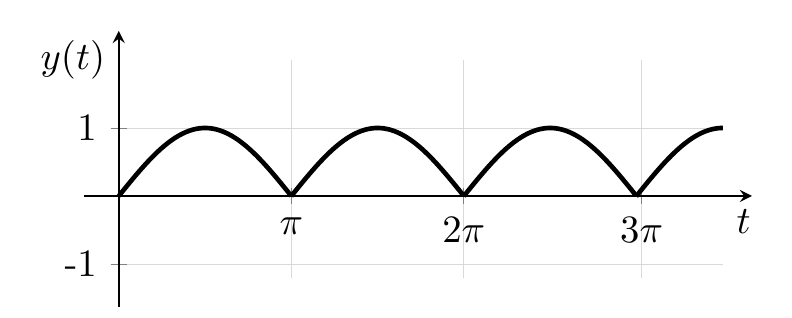
\begin{tikzpicture}[scale=1.4] 
            \begin{axis}[
            width=2.8in,
            height=1.4in,
            clip=false,
            axis lines=middle,
            xmin=-.1,xmax=11,
            ymin=-1.2, ymax=2,
            xtick={3.14,6.28,9.52},
            xticklabels={$\pi$,$2\pi$,$3\pi$},
            ytick={-1,0,1},
            yticklabels={-1,0,1},        
            axis line style={shorten >=-7.5pt, shorten <=-7.5pt},
            xlabel=$t$,
            ylabel=$y(t)$,
            xlabel style={at={(ticklabel* cs:1)},anchor=north west},
            ylabel style={at={(ticklabel* cs:1)},anchor= east},
            grid style={line width=.2pt, draw=gray!30},
            grid=both,
            ]
            \addplot[black,samples=50,domain=0:3.1415,very thick] {sin(deg(x))};% 
            \addplot[black,samples=50,domain=3.14:6.28,very thick] {sin(deg(x)-180)};% 
            \addplot[black,samples=50,domain=6.28:9.42,very thick] {sin(deg(x)-360)};% 
            \addplot[black,samples=50,domain=9.42:11,very thick] {sin(deg(x)-180)};% 
            \end{axis}
        \end{tikzpicture} 
        \end{center}
        
        Over the interval from $0$ to $\pi$, $y(t)=\sin(t)$. The function $y$ is defined for $t \ge 0$. Calculate the Laplace transform of the periodic function $y(t)$. Do not leave your work in terms of integrals and show your work. 
    
\newpage \Initials

    \question[10] Use the Laplace transform to solve the following IVP.

    % $$\displaystyle y''-4y'+4y=0,\qquad y(0)=1,\quad y'(0)=1$$ %Q,A HW 5.4#4
    % $$\displaystyle y''-2y'+4y=0,\qquad y(0)=2,\quad y'(0)=0$$ %M HW 5.4#5
    
    % $$ y'' -6y'+13y = 0, \quad y(0) = 0, \quad y'(0) = -3$$. % A TRIM P301 #27
    $$ y''+ 2y'+y = 0, \quad y(0) = 1, \quad y'(0) = 1$$. % B TRIM P301 #23
    

\newpage \Initials

    \question[10] Use the Laplace transform to solve the following IVP.

    % $$\displaystyle y''-y=10\delta(t-4)\qquad y(0)=3,\quad y'(0)=3 $$ %A WORKSHEET 5.7#1 %%% SP19
    % $$\displaystyle y''+4y=10\delta(t-4\pi)\qquad y(0)=\frac12,\quad y'(0)=0 $$ %Q 5.7#6 %%% SP19
    % $$\displaystyle y''+2y'+2y=10\delta(t-\pi)\qquad y(0)=0,\quad y'(0)=1 $$ %M 5.7#1 %%% SP19

    $$y'' + 2y' = \delta(t-1), \quad y(0) = 0, \quad y'(0) = 1$$ % TRIM PAGE 318

\newpage \Initials
    
    \question[2] A small number of points will be allocated for presentation, neatness, and organization. Please ensure that
    \begin{enumerate}
        % \item your scan is under 5 MB in file size
        \item your work is legible in the scan
        \item your name or initials are at the top of every page
        \item questions are answered in the order in which they were given
        \item during the upload process you have indicated which pages correspond to which question, and made sure that none of your pages are upside down or sideways (you can also change the orientation of the pages when you upload in Gradescope)
    \end{enumerate}
    Ensuring that these criteria are met helps ensure that your exam is graded efficiently and accurately. 
    


    
\end{questions}
    
    Please sign and date the following GT Honor Code statement. \\ 
    \vspace{2pt}
    
    \textbf{Georgia Tech Honor Code}:\ \GTHonorCode
    
    \begin{center}
    \begin{center}
        \def\arraystretch{0.35}%  1 is the default, change whatever you need
        \begin{tabular}{ b{8cm} b{8cm} }
        \vspace{.5cm} \underline{\hspace{7cm}} & \vspace{.5cm} \underline{\hspace{4.5cm}}  \tabularnewline
        \vspace{6pt} signature & \vspace{6pt} date    
        \end{tabular}
    \end{center}
    \end{center}    
\end{document}
